%El método desarrollado y preferido por Celera se llama 
%simplemente secuenciación shotgun. Este enfoque fue desarrollado 
%y perfeccionado en los genomas procariotas que son más pequeños en
% tamaño y contienen ADN menos repetitivas. secuenciación aleatoria
% escopeta cizalla ADN genómico en trozos pequeños que están clonados
% en plásmidos y secuenciado en ambas cadenas, lo que elimina el paso
% de BAC del planteamiento del PGH es. Una vez que las secuencias se 
%obtienen, son alineados y montados en la secuencia final.

\frame
{
\begin{center}
	\Huge{Técnicas}\\
	\huge{Shotgun Sequencing}
\end{center}
}

\frame
{
\frametitle{Shotgun Sequencing}
\framesubtitle{¿Qué es?}

\begin{itemize}
	\item Método de secuenciado de ADN, desarrollado y preferido por ``Celera Genomics'', una empresa estadounidense.
	\item Conocido también como ``shotgun cloning''
\end{itemize}

}

\frame
{
\frametitle{Shotgun Sequencing}
\framesubtitle{Ventajas y Desventajas}

\begin{itemize}
	\item Ventajas:
		\begin{itemize}
			\item Moderadamente rápido en procesamiento
		\end{itemize}
	\item Desventajas:
		\begin{itemize}
			\item Problemas con secuencias con repetición.
			\item No detecta secuencias repetidas. Para aquello se basa en datos públicos.
		\end{itemize}
\end{itemize}

}

\frame
{
\frametitle{Shotgun Sequencing}
\framesubtitle{Descripción}
\begin{center}
	\huge{Video}	
\end{center}

}

\frame
{
\frametitle{Shotgun Sequencing}
\framesubtitle{Descripción}

Tomando como ejemplo un genoma trozado en 9 partes:\\

\begin{center}
	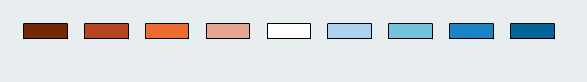
\includegraphics[width=0.5\textwidth]{img/tecnica1-1.png}
\end{center}
}

\frame
{
\frametitle{Shotgun Sequencing}
\framesubtitle{Descripción}

\begin{center}
	\huge ¿Cuantas posibles combinaciones podemos formar?
\end{center}
}

\frame
{
\frametitle{Shotgun Sequencing}
\framesubtitle{Descripción}

\begin{center}
	\huge $9 * 8 * 7 * ... * 2 * 1 = 9! = 362880$
\end{center}
}

\frame
{
\frametitle{Shotgun Sequencing}
\framesubtitle{Descripción}

Dejando de lado la cantidad.\\

\begin{center}
	\huge ¿Como saber cual es la combinación correcta?
\end{center}
}

\frame
{
\frametitle{Shotgun Sequencing}
\framesubtitle{Descripción}

\begin{center}
	
\includegraphics[width=0.5\textwidth]{img/tecnica1-2.png}
\end{center}

}

\frame
{
\frametitle{Shotgun Sequencing}
\framesubtitle{Descripción}

\begin{center}
	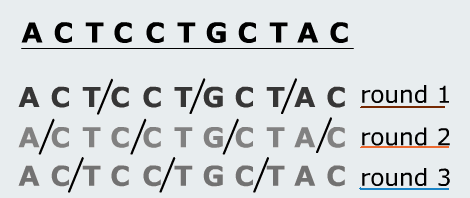
\includegraphics[width=0.5\textwidth]{img/tecnica1-3.png}
\end{center}

}

\frame
{
\frametitle{Shotgun Sequencing}
\framesubtitle{Descripción}

\begin{center}
	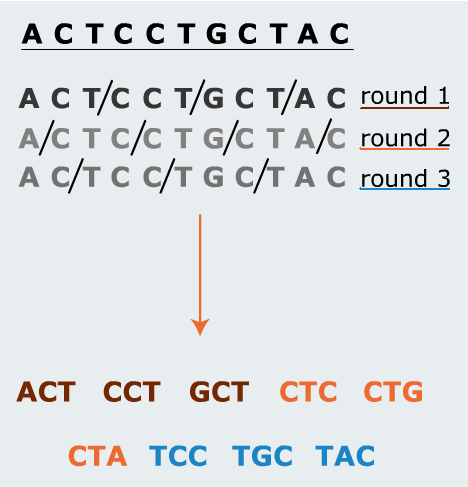
\includegraphics[width=0.5\textwidth]{img/tecnica1-4.png}
\end{center}

}

\frame
{
\frametitle{Shotgun Sequencing}
\framesubtitle{Descripción}

Luego se crea un grafo dirigido:

\begin{itemize}
	\item Sea $x_i = c_{i1} c_{i2} ... c_{in-1} c_{in}$ el contenido de un estado $i$ en el grafo
	\item Para ir de un estado $i$ a un estado $j$, es necesario que: $x_{in-1}x_{in} = x_{j1} x_{j2}$
	\item Finalmente se busca un ciclo hamiltoneano en dicho grafo, correspondiente a la secuencia buscada.
\end{itemize}
}


\frame
{
\frametitle{Shotgun Sequencing}
\framesubtitle{Descripción}

\begin{center}
	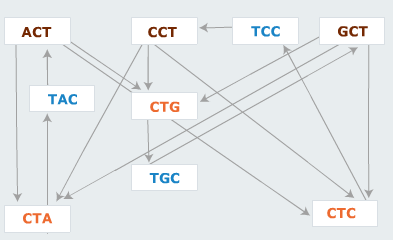
\includegraphics[width=0.7\textwidth]{img/tecnica1-5.png}
\end{center}

}

\frame
{
\frametitle{Shotgun Sequencing}
\framesubtitle{Descripción}

\begin{center}
	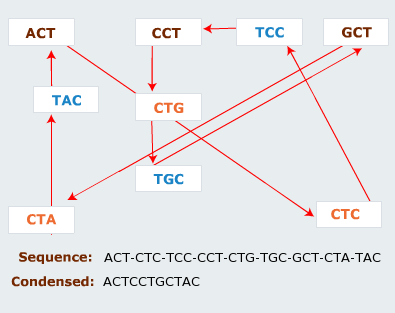
\includegraphics[width=0.7\textwidth]{img/tecnica1-6.png}
\end{center}
}
